\chapter{Alternative points prescription for theory error}
\label{app:the_error_3pt}
In sec.~\ref{sec:scale_var} we have discussed how to construct the theory covariance matrix using the so-called 9-points prescription, 
where the renormalization and factorization scales of a specific process are varied completely independently.
In ref.~\cite{AbdulKhalek:2019ihb} a series of alternative options are investigated, and the 9-points prescription is selected 
as the most suitable one according to the validation procedure described in sec.~\ref{sec:validation}.
In this appendix we present an alternative simpler choice, denoted as 3-points prescription,
studying how the fit and validation results change, and showing how the 9-points prescription is indeed a better option. 

%
In the 3-points prescription both the renormalization and factorization scales are varied coherently by a fixed amount about the
central value.
In other words, considering a single process we set $k_f=k_r$ and we only vary the single resulting scale, obtaining the
2+1 points in the scales space shown in Fig.~\ref{fig:3-points}.
\begin{figure}[t]
    \centering
    {\begin{tikzpicture}
    \draw[->] (-1.5,0) -- (1.5,0);
    \draw[->] (0,-1.5) -- (0,1.5);
    \filldraw[black] (0,0) circle (2pt);
    \filldraw[black] (-1,-1) circle (2pt);
    \filldraw[black] (1,1) circle (2pt);
    \node at (0.5,1.5) {$\kappa_{r}$};
    \node at (1.9,0) {$\kappa_f$};
    \end{tikzpicture}}\qquad
    \begin{caption}{3-points prescription for a single process.}
      \label{fig:3-points}
    \end{caption}
\end{figure}
The resulting entries for the theory covariance matrix are 
\begin{align}
    \label{3S}
    S^{(\rm 3pt)}_{ij} = \frac{1}{2}\big\{ \Delta_i^{++}\Delta_j^{++}  + \Delta_i^{--}\Delta_j^{--}\big\} \, ,
\end{align}
where the indices $i,j$ label point belonging to the same process $\pi$.
Considering two different processes $\pi_1$ and $\pi_2$ we set $k_f=k_{r_1}$ for $\pi_1$ and $k_f=k_{r_1}$ for $\pi_2$
and then vary $k_{r_1}$ and $k_{r_2}$ independently. Note that in this way the correlation in the variation of $k_f$
between $\pi_1$ and $\pi_2$ is necessarily ignored so that the variations for each process are entirely uncorrelated.
eq.~\eqref{3S} is generalized to the off-diagonal entries of the theory covariance matrix getting
\begin{equation}
    S^{(\rm 3pt)}_{i_1j_2} = 
    \frac{1}{4}\big\{\big(\Delta_{i_1}^{++} + \Delta_{i_1}^{--} \big) \big(\Delta_{j_2}^{++} + \Delta_{j_2}^{--} \big) \big\}\, ,
\end{equation}
where the indices $i_1,j_2$ now label point belonging to the processes $\pi_1$ and $\pi_2$ respectively.
The validation of such covariance matrix proceeds like described in sec.~\ref{sec:validation},
through the computation of the angle $\theta$ between the shift $\delta$ and its component on the
subspace $S$, defined in eq.~\eqref{eq:angle}. In Table ~\ref{tab:process_efficiencies} 
we compare the values of such angle for each process in the case of the 3- and 9-points prescriptions.
We note how the former performs rather poorly in comparison to the 9-points one,
suggesting that the lack of correlation in the factorization scale between processes in this prescription
implies that much of the correlation pattern in the MHOU due to universal PDF evolution has been missed.
\begin{table}[ht!]
	\centering
	\small
	%%%%%%%%%%%%%%%%%%%%%%%%%%%%%%%%%%%%%%%%%%%%%%%%%%%%%%%%%%%
\renewcommand*{\arraystretch}{1.20}
\begin{tabular}{|c|c|c|c|c|c|c|c|}
 \toprule
%\cline{3-7}
% \multicolumn{5}{c|}{$\theta$} \\
Presc. & $N_{\rm sub}$ & DIS NC & DIS CC & DY & JET & TOP \\
\cline{3-7}
& & 1593 & 552 & 484 & 164 & 26 \\
\hline
 5-pt & 4 &39$^{\rm o}$ & 21$^{\rm o}$ & 25$^{\rm o}$ & 17$^{\rm o}$ & 11$^{\rm o}$	\\
$\overline{5}$-pt & 4 & 38$^{\rm o}$ & 17$^{\rm o}$ & 23$^{\rm o}$	& 22$^{\rm o}$ & 10$^{\rm o}$ \\
9-pt & 8 & 32$^{\rm o}$ & 16$^{\rm o}$ & 22$^{\rm o}$ & 14$^{\rm o}$ & 3$^{\rm o}$	\\
\hline
 3-pt & 2 &54$^{\rm o}$ & 36$^{\rm o}$ & 39$^{\rm o}$ & 24$^{\rm o}$ & 12$^{\rm o}$ \\
7-pt & 6 &35$^{\rm o}$ & 17$^{\rm o}$ & 22$^{\rm o}$ & 16$^{\rm o}$ & 3$^{\rm o}$	\\
    \bottomrule
\end{tabular}
%%%%%%%%%%%%%%%%%%%%%%%%%%%%%%%%%%%%%%%%%%%%%%%%%%%%%%%%%%%%%%%%%%

        \vspace{3mm}
	\caption{Comparison between the $\theta$ values for the 3- and 9-points prescriptions.}
	\label{tab:process_efficiencies}
\end{table}

%
In Table.~\ref{tab:chi_3_vs_9} we compare the values for the total $\chi^2$ and $\phi$ estimator for fits performed with the 9-points,
already shown in sec.~\ref{sec:th_error_results}, and the 3-points
prescription, together with values for the baseline NLO fit produced without any theory error.
Unlike the 9-points prescription case, for which as observed in sec.~\ref{sec:th_error_results}
the $\chi^2$ improves with respect to the baseline,
in the case of the 3-points prescription the fit quality remains unchanged after the inclusion of the MHOU.
Both prescriptions show an increase in the value of $\phi$, which is bigger in the case of the 9-points one.

\begin{table}[ht!]
	\centering
	\small
	%%%%%%%%%%%%%%%%%%%%%%%%%%%%%%%%%%%%%%%%%%%%%%%%%%%%%%%%%%%
\renewcommand*{\arraystretch}{1.20}
\begin{tabular}{|c|c|c|c|}
 \toprule
%\cline{3-7}
% \multicolumn{5}{c|}{$\theta$} \\
	 &  $C$ & $C+S^{\rm(3pt)}$ & $C+S^{\rm (9pt)}$ \\
\hline
$\chi^2$  & 1.139  & 1.139 & 1.109 	\\
\hline
$\phi$  & 0.314  & 0.394  & 0.405   \\
\bottomrule
\end{tabular}
%%%%%%%%%%%%%%%%%%%%%%%%%%%%%%%%%%%%%%%%%%%%%%%%%%%%%%%%%%%%%%%%%%

        \vspace{3mm}
	\caption{Comparison between $\chi^2$ and $\phi$ total values of 3- and 9-points prescriptions}
	\label{tab:chi_3_vs_9}
\end{table}

%
Finally in Fig.~\ref{fig:pdfs_plots_th_err_3_vs_9} we study the dependence of the fit results on the choice of the prescription
for the theory covariance matrix, taking as example the gluon distribution. In the same plot we report also the central value of
the NNLO fit with experimental uncertainties only and all the distributions are normalized to the 3-points prescription results.
In general the two results are consistent, but the central value of the 9-points prescription result is much closer 
to the NNLO central value, providing further confirmation for preferring the 9-point prescription.

\begin{figure}[t!]
    \begin{center}
        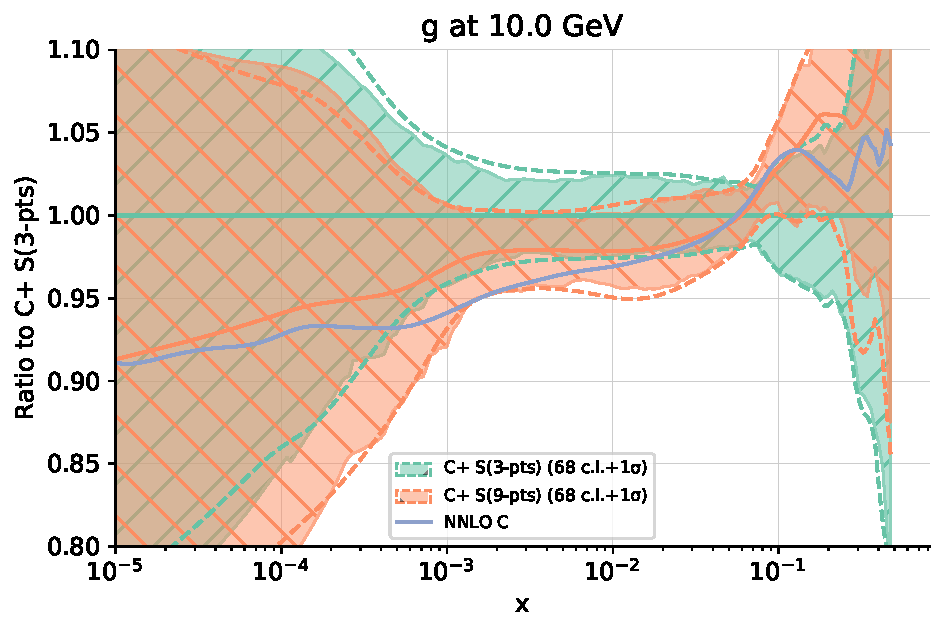
\includegraphics[width=0.49\linewidth]{plot_pdfs_g_3_vs_9.pdf}
        \caption{Comparison between the gluon PDF produced using the 3-points and 9-points prescription
        for the theory covariance matrix. The central value of the NNLO fit without any theory error is also shown.
        All the distributions are normalized to the 3-points prescription results.} 
        \label{fig:pdfs_plots_th_err_3_vs_9} 
    \end{center}
\end{figure}